\documentclass[a4paper,12pt]{article}
\usepackage[latin1]{inputenc}
%\usepackage[spanish]{babel}
\usepackage{bm}
\usepackage{graphicx}
\usepackage{amsmath}
\usepackage{tikz}
\usepackage{pgfplots}
\usepackage{pgfplotstable}
\usetikzlibrary{quotes,angles}
\usetikzlibrary{shapes.geometric}
\usetikzlibrary{arrows}
\usepackage{textcomp}
\setlength{\textheight}{235mm}
\setlength{\textwidth}{168mm}
\setlength{\oddsidemargin}{0pt}
\pagestyle{empty}
\begin{document}
\mbox{}\vspace*{-45mm}

{\centering
{\small\sc Escuela T�cnica Superior de Ingenieros de Caminos, Canales y
Puertos (Madrid)}\\*[4mm]
{\Large\bf M�todo de los Elementos Finitos. Examen extraordinario (26/01/2023)}\\*[4mm]
Ejercicio 1: Estructura de barras articuladas \\*[4mm]
}

\vspace{3mm}

%%%%%
\noindent

Se tiene la estructura de barras articuladas (viga Pratt) mostrada en la Figura~\ref{fig:pratt}. El m�dulo de elasticidad es $E= 210\,\mbox{GPa}$. El �rea de la secci�n transversal es $A=20\cdot 10^3\,\mbox{mm}^2$. 

Las dimensiones, condiciones de contorno de la estructura y cargas aplicadas se indican en la figura. 

Se pide hacer un modelo de elementos finitos que permita conocer la respuesta mec�nica de la estructura y contestar el cuestionario. 

\begin{figure}[htpb]
\centering
 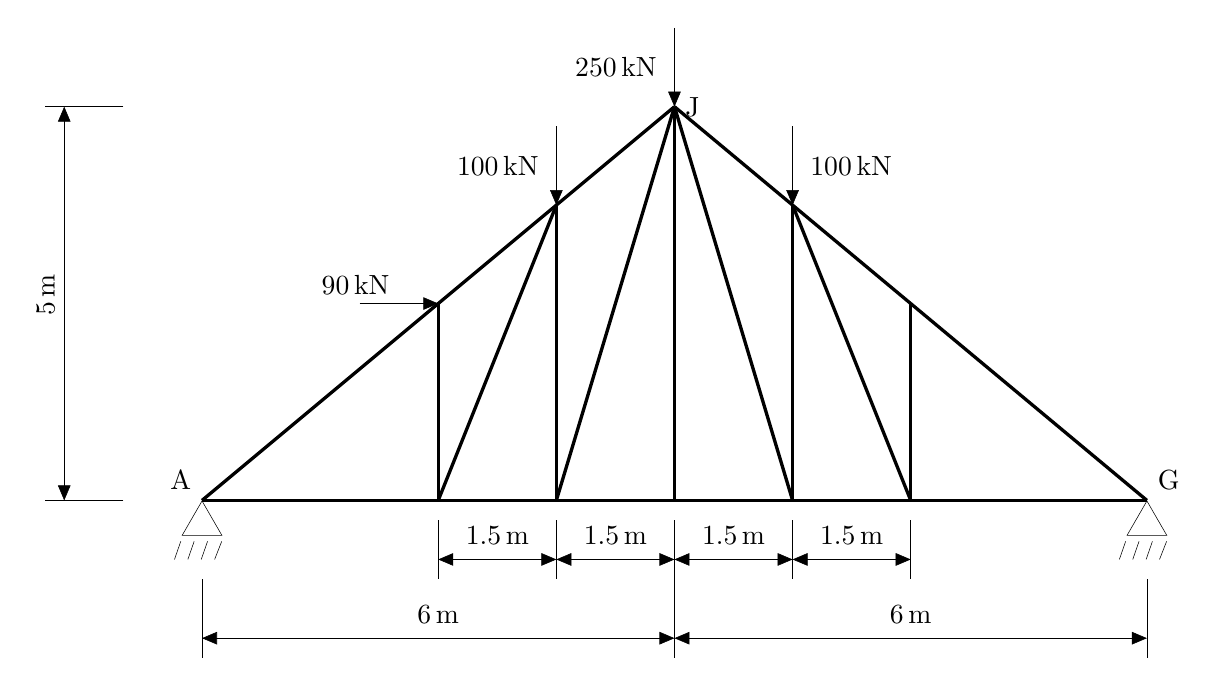
\begin{tikzpicture}[>=triangle 45]
 %XYplane
\draw[very thick,-] (0,0) node(origin)[anchor=south east]{A} -- (12,0) node[anchor=south west] {G};
\draw[very thick,-] (0,0) -- (6,5) node[anchor=west]{J};
\draw[very thick,-] (12,0) -- (6,5);
\draw[very thick,-] (3,0) -- (3,2.50);
\draw[very thick,-] (9,0) -- (9,2.50);
\draw[very thick,-] (4.5,0) -- (4.5,3.75);
\draw[very thick,-] (7.5,0) -- (7.5,3.75);
\draw[very thick,-] (6,0) -- (6,5);
\draw[very thick,-] (4.5,3.75) -- (3,0);
\draw[very thick,-] (6,5) -- (4.5,0);
\draw[very thick,-] (6,5) -- (7.5,0);
\draw[very thick,-] (7.5,3.75) -- (9,0);

%cargas
\draw[very thin,->] (6,6) -- node[left=3]{$250\,\mbox{kN}$}(6,5);
\draw[very thin,->] (4.5,4.75) -- node[left=3]{$100\,\mbox{kN}$}(4.5,3.75);
\draw[very thin,->] (7.5,4.75) -- node[right=3]{$100\,\mbox{kN}$}(7.5,3.75);
\draw[very thin,->] (2.0,2.5) -- node[above left]{$90\,\mbox{kN}$}(3,2.5);

%apoyos
\node[isosceles triangle, isosceles triangle apex angle=60, draw,very thin ,rotate=90, minimum size =0.15cm, anchor=apex] (T) at (0,0){};
\node[isosceles triangle, isosceles triangle apex angle=60, draw, very thin, rotate=90, minimum size =0.15cm, anchor=apex] (T1) at (12,0){};
\draw[very thin,-] (-0.27,-0.52) -- (-0.35,-0.75);
\draw[very thin,-] (-0.10,-0.52) -- (-0.18,-0.75);
\draw[very thin,-] (0.07,-0.52) -- (-0.01,-0.75);
\draw[very thin,-] (0.25,-0.52) -- (0.16,-0.75);

\draw[very thin,-] (12-0.27,-0.52) -- (12-0.35,-0.75);
\draw[very thin,-] (12-0.10,-0.52) -- (12-0.18,-0.75);
\draw[very thin,-] (12+0.07,-0.52) -- (12-0.01,-0.75);
\draw[very thin,-] (12+0.25,-0.52) -- (12+0.16,-0.75);

%cotas
\draw[very thin,-] (-1,0) -- (-2,0);
\draw[very thin,-] (-1,5) -- (-2,5);

\draw[very thin,<->] (-1.75,0) -- node[above=3,rotate=90]{$5\,\mbox{m}$}(-1.75,5);

\draw[very thin,-] (0,-1) -- (0,-2);
\draw[very thin,-] (12,-1) -- (12,-2);
\draw[very thin,-] (6,-0.25) -- (6,-2);

\draw[very thin,-] (3,-0.25) -- (3,-1);
\draw[very thin,-] (4.5,-0.25) -- (4.5,-1);
\draw[very thin,-] (7.5,-0.25) -- (7.5,-1);
\draw[very thin,-] (9,-0.25) -- (9,-1);

\draw[very thin,<->] (0,-1.75) -- node[above=2]{$6\,\mbox{m}$}(6,-1.75);
\draw[very thin,<->] (6,-1.75) -- node[above=2]{$6\,\mbox{m}$}(12,-1.75);

\draw[very thin,<->] (3,-0.75) -- node[above=2]{$1.5\,\mbox{m}$}(4.5,-0.75);
\draw[very thin,<->] (4.5,-0.75) -- node[above=2]{$1.5\,\mbox{m}$}(6,-0.75);
\draw[very thin,<->] (6,-0.75) -- node[above=2]{$1.5\,\mbox{m}$}(7.5,-0.75);
\draw[very thin,<->] (7.5,-0.75) -- node[above=2]{$1.5\,\mbox{m}$}(9,-0.75);



\end{tikzpicture}
\caption{Geometr�a y cargas de la viga.} 
\label{fig:pratt}
\end{figure}

\end{document}
